%% uncomment to list all files in log
%\listfiles

\documentclass[12pt]{report}


\usepackage{fontspec}

%\setmainfont[Scale=MatchLowercase]{Lucida Bright}
%\setmonofont{FreeMono}
%\setmonofont{Source Code Pro}
\setmonofont[Scale=MatchLowercase]{Ubuntu Mono}

\usepackage[headings]{fullpage}

% national use characters 
%\usepackage{inputenc}

% ams mathematical symbols
\usepackage{amsmath,amssymb}

% added to support pandoc highlighting
\usepackage{microtype}

\usepackage{makeidx}

% add index and bibliographies to table of contents
\usepackage[nottoc]{tocbibind}

% postscript courier and times in place of cm fonts
%\usepackage{courier}
%\usepackage{times}

% extended coloring
\usepackage{color}
\usepackage[table,dvipsnames]{xcolor}
\usepackage{colortbl}

% advanced date formating
\usepackage{datetime}

%support pandoc code highlighting
\usepackage{fancyvrb}
\DefineShortVerb[commandchars=\\\{\}]{\|}
\DefineVerbatimEnvironment{Highlighting}{Verbatim}{commandchars=\\\{\}}
% Add ',fontsize=\small' for more characters per line

%tango style colors
% \usepackage{framed}
% \definecolor{shadecolor}{RGB}{255,255,255}
% \newenvironment{Shaded}{\begin{snugshade}}{\end{snugshade}}
% \newcommand{\KeywordTok}[1]{\textcolor[rgb]{0.13,0.29,0.53}{\textbf{{#1}}}}
% \newcommand{\DataTypeTok}[1]{\textcolor[rgb]{0.13,0.29,0.53}{{#1}}}
% \newcommand{\DecValTok}[1]{\textcolor[rgb]{0.00,0.00,0.81}{{#1}}}
% \newcommand{\BaseNTok}[1]{\textcolor[rgb]{0.00,0.00,0.81}{{#1}}}
% \newcommand{\FloatTok}[1]{\textcolor[rgb]{0.00,0.00,0.81}{{#1}}}
% \newcommand{\CharTok}[1]{\textcolor[rgb]{0.31,0.60,0.02}{{#1}}}
% \newcommand{\StringTok}[1]{\textcolor[rgb]{0.31,0.60,0.02}{{#1}}}
% \newcommand{\CommentTok}[1]{\textcolor[rgb]{0.56,0.35,0.01}{\textit{{#1}}}}
% \newcommand{\OtherTok}[1]{\textcolor[rgb]{0.56,0.35,0.01}{{#1}}}
% \newcommand{\AlertTok}[1]{\textcolor[rgb]{0.94,0.16,0.16}{{#1}}}
% \newcommand{\FunctionTok}[1]{\textcolor[rgb]{0.00,0.00,0.00}{{#1}}}
% \newcommand{\RegionMarkerTok}[1]{{#1}}
% \newcommand{\ErrorTok}[1]{\textbf{{#1}}}
% \newcommand{\NormalTok}[1]{{#1}}

%espresso style colors
% \usepackage{framed}
% \definecolor{shadecolor}{RGB}{42,33,28}
% \newenvironment{Shaded}{\begin{snugshade}}{\end{snugshade}}
% \newcommand{\KeywordTok}[1]{\textcolor[rgb]{0.26,0.66,0.93}{\textbf{{#1}}}}
% \newcommand{\DataTypeTok}[1]{\textcolor[rgb]{0.74,0.68,0.62}{\underline{{#1}}}}
% \newcommand{\DecValTok}[1]{\textcolor[rgb]{0.27,0.67,0.26}{{#1}}}
% \newcommand{\BaseNTok}[1]{\textcolor[rgb]{0.27,0.67,0.26}{{#1}}}
% \newcommand{\FloatTok}[1]{\textcolor[rgb]{0.27,0.67,0.26}{{#1}}}
% \newcommand{\CharTok}[1]{\textcolor[rgb]{0.02,0.61,0.04}{{#1}}}
% \newcommand{\StringTok}[1]{\textcolor[rgb]{0.02,0.61,0.04}{{#1}}}
% \newcommand{\CommentTok}[1]{\textcolor[rgb]{0.00,0.40,1.00}{\textit{{#1}}}}
% \newcommand{\OtherTok}[1]{\textcolor[rgb]{0.74,0.68,0.62}{{#1}}}
% \newcommand{\AlertTok}[1]{\textcolor[rgb]{1.00,1.00,0.00}{{#1}}}
% \newcommand{\FunctionTok}[1]{\textcolor[rgb]{1.00,0.58,0.35}{\textbf{{#1}}}}
% \newcommand{\RegionMarkerTok}[1]{\textcolor[rgb]{0.74,0.68,0.62}{{#1}}}
% \newcommand{\ErrorTok}[1]{\textcolor[rgb]{0.74,0.68,0.62}{\textbf{{#1}}}}
% \newcommand{\NormalTok}[1]{\textcolor[rgb]{0.74,0.68,0.62}{{#1}}}

%kete style colors
% \newenvironment{Shaded}{}{}
% \newcommand{\KeywordTok}[1]{\textbf{{#1}}}
% \newcommand{\DataTypeTok}[1]{\textcolor[rgb]{0.50,0.00,0.00}{{#1}}}
% \newcommand{\DecValTok}[1]{\textcolor[rgb]{0.00,0.00,1.00}{{#1}}}
% \newcommand{\BaseNTok}[1]{\textcolor[rgb]{0.00,0.00,1.00}{{#1}}}
% \newcommand{\FloatTok}[1]{\textcolor[rgb]{0.50,0.00,0.50}{{#1}}}
% \newcommand{\CharTok}[1]{\textcolor[rgb]{1.00,0.00,1.00}{{#1}}}
% \newcommand{\StringTok}[1]{\textcolor[rgb]{0.87,0.00,0.00}{{#1}}}
% \newcommand{\CommentTok}[1]{\textcolor[rgb]{0.50,0.50,0.50}{\textit{{#1}}}}
% \newcommand{\OtherTok}[1]{{#1}}
% \newcommand{\AlertTok}[1]{\textcolor[rgb]{0.00,1.00,0.00}{\textbf{{#1}}}}
% \newcommand{\FunctionTok}[1]{\textcolor[rgb]{0.00,0.00,0.50}{{#1}}}
% \newcommand{\RegionMarkerTok}[1]{{#1}}
% \newcommand{\ErrorTok}[1]{\textcolor[rgb]{1.00,0.00,0.00}{\textbf{{#1}}}}
% \newcommand{\NormalTok}[1]{{#1}}
%end pandoc code hacks

% jodliterate colors
\usepackage{color}
\definecolor{shadecolor}{RGB}{248,248,248}
% j control structures 
\definecolor{keywcolor}{rgb}{0.13,0.29,0.53}
% j explicit arguments x y m n u v
\definecolor{datacolor}{rgb}{0.13,0.29,0.53}
% j numbers - all types see j.xml
\definecolor{decvcolor}{rgb}{0.00,0.00,0.81}
\definecolor{basencolor}{rgb}{0.00,0.00,0.81}
\definecolor{floatcolor}{rgb}{0.00,0.00,0.81}
% j local assignments
\definecolor{charcolor}{rgb}{0.31,0.60,0.02}
\definecolor{stringcolor}{rgb}{0.31,0.60,0.02}
\definecolor{commentcolor}{rgb}{0.56,0.35,0.01}
% primitive adverbs and conjunctions
%\definecolor{othercolor}{rgb}{0.56,0.35,0.01}   
\definecolor{othercolor}{RGB}{0,0,255}
% global assignments
\definecolor{alertcolor}{rgb}{0.94,0.16,0.16}
% primitive J verbs and noun names
\definecolor{funccolor}{rgb}{0.00,0.00,0.00}    

\usepackage{framed}
\newenvironment{Shaded}{}{}
\newcommand{\KeywordTok}[1]{\textcolor{keywcolor}{\textbf{{#1}}}}
\newcommand{\DataTypeTok}[1]{\textcolor{datacolor}{{#1}}}
%\newcommand{\DecValTok}[1]{\textcolor{decvcolor}{{#1}}}
\newcommand{\DecValTok}[1]{{#1}} 
\newcommand{\BaseNTok}[1]{\textcolor{basencolor}{{#1}}}
\newcommand{\FloatTok}[1]{\textcolor{floatcolor}{{#1}}}
\newcommand{\CharTok}[1]{\textcolor{charcolor}{\textbf{{#1}}}}
\newcommand{\StringTok}[1]{\textcolor{stringcolor}{{#1}}}
\newcommand{\CommentTok}[1]{\textcolor{commentcolor}{\textit{{#1}}}}
\newcommand{\OtherTok}[1]{\textcolor{othercolor}{{#1}}} 
\newcommand{\AlertTok}[1]{\textcolor{alertcolor}{\textbf{{#1}}}}
%\newcommand{\FunctionTok}[1]{\textcolor{funccolor}{{#1}}}
\newcommand{\FunctionTok}[1]{{#1}}
\newcommand{\RegionMarkerTok}[1]{{#1}}
\newcommand{\ErrorTok}[1]{\textbf{{#1}}}
\newcommand{\NormalTok}[1]{{#1}}

% headers and footers
\usepackage{fancyhdr}
\pagestyle{fancy}

\fancyhead{}
\fancyfoot{}

%\fancyhead[LE,RO]{\slshape \rightmark}
%\fancyhead[LO,RE]{\slshape \leftmark}
\fancyfoot[C]{\thepage}
%\headrulewidth 0.4pt
%\footrulewidth 0 pt

%\addtolength{\headheight}{\baselineskip}

%\lfoot{\emph{Analyze the Data not the Drivel}}
%\rfoot{\emph{\today}}

% subfigure handles figures that contain subfigures
%\usepackage{color,graphicx,subfigure,sidecap}
\usepackage{graphicx,sidecap}
\usepackage{subfigure}
\graphicspath{{./inclusions/}}

% floatflt provides for text wrapping around small figures and tables
\usepackage{floatflt}

% tweak caption formats 
\usepackage{caption} 
\usepackage{sidecap}
%\usepackage{subcaption} % not compatible with subfigure

\usepackage{rotating} % flip tables sideways

% complex footnotes
%\usepackage{bigfoot}

% weird logos \XeLaTeX
\usepackage{metalogo}

% source code listings
\usepackage{listings}

% long tables
% \usepackage{longtable}

\newcommand{\HRule}{\rule{\linewidth}{0.5mm}}

% map LaTeX cross references into PDF cross references
\usepackage[
            %dvips,
            colorlinks,
            linkcolor=blue,
            citecolor=blue,
            urlcolor=blue,   % magenta, cyan default        
            pdfauthor={John D. Baker},
            pdftitle={Analyze the Data not the Drivel},
            pdfsubject={Blog},
            pdfcreator={MikTeX+LaTeXe with hyperref package},
            pdfkeywords={blog,wordpress},
            ]{hyperref}
           
% custom colors
\definecolor{CodeBackGround}{cmyk}{0.0,0.0,0,0.05}    % light gray
\definecolor{CodeComment}{rgb}{0,0.50,0.00}           % dark green {0,0.45,0.08}
\definecolor{TableStripes}{gray}{0.9}                 % odd/even background in tables

\lstdefinelanguage{bat}
{morekeywords={echo,title,pushd,popd,setlocal,endlocal,off,if,not,exist,set,goto,pause},
sensitive=True,
morecomment=[l]{rem}
}

\lstdefinelanguage{jdoc}
{
morekeywords={},
otherkeywords={assert.,break.,continue.,for.,do.,if.,else.,elseif.,return.,select.,end.
,while.,whilst.,throw.,catch.,catchd.,catcht.,try.,case.,fcase.},
sensitive=True,
morecomment=[l]{NB.},
morestring=[b]',
morestring=[d]',
}

% latex size ordering - can never remember it
% \tiny
% \scriptsize
% \footnotesize
% \small
% \normalsize
% \large
% \Large
% \LARGE
% \huge
% \Huge
 
% listings package settings  
\lstset{%
  language=jdoc,                                % j document settings
  basicstyle=\ttfamily\footnotesize,            
  keywordstyle=\bfseries\color{keywcolor}\footnotesize,
  identifierstyle=\color{black},
  commentstyle=\slshape\color{CodeComment},     % colored slanted comments
  stringstyle=\color{red}\ttfamily,
  showstringspaces=false,                       
  %backgroundcolor=\color{CodeBackGround},       
  frame=single,                                
  framesep=1pt,                                 
  framerule=0.8pt,                             
  rulecolor=\color{CodeBackGround},   
  showspaces=false,
  %columns=fullflexible,
  %numbers=left,
  %numberstyle=\footnotesize,
  %numbersep=9pt,
  tabsize=2,
  showtabs=false,
  captionpos=b
  breaklines=true,                              
  breakindent=5pt                              
}

\lstdefinelanguage{JavaScript}{
  keywords={typeof, new, true, false, catch, function, return, null, catch, switch, var, if, in, while, do, else, case, break},
  ndkeywords={class, export, boolean, throw, implements, import, this},
  ndkeywordstyle=\color{darkgray}\bfseries,
  sensitive=false,
  comment=[l]{//},
  morecomment=[s]{/*}{*/},
  morestring=[b]',
  morestring=[b]"
}

% C# settings
\lstdefinestyle{sharpc}{
language=[Sharp]C,
basicstyle=\ttfamily\scriptsize, 
keywordstyle=\bfseries\color{keywcolor}\scriptsize,
framerule=0pt
}

% for source code listing longer than two use smaller font
\lstdefinestyle{smallersource}{
basicstyle=\ttfamily\scriptsize, 
keywordstyle=\bfseries\color{keywcolor}\scriptsize,
framerule=0pt
}

\lstdefinestyle{resetdefaults}{
language=jdoc,
basicstyle=\ttfamily\footnotesize,  
keywordstyle=\bfseries\color{keywcolor}\footnotesize,                                                               
framerule=0.8pt 
}

% APL UTF8 code points listed for lstlisting processing
\makeatletter
\lst@InputCatcodes
\def\lst@DefEC{%
 \lst@CCECUse \lst@ProcessLetter
  ^^80^^81^^82^^83^^84^^85^^86^^87^^88^^89^^8a^^8b^^8c^^8d^^8e^^8f%
  ^^90^^91^^92^^93^^94^^95^^96^^97^^98^^99^^9a^^9b^^9c^^9d^^9e^^9f%
  ^^a0^^a1^^a2^^a3^^a4^^a5^^a6^^a7^^a8^^a9^^aa^^ab^^ac^^ad^^ae^^af%
  ^^b0^^b1^^b2^^b3^^b4^^b5^^b6^^b7^^b8^^b9^^ba^^bb^^bc^^bd^^be^^bf%
  ^^c0^^c1^^c2^^c3^^c4^^c5^^c6^^c7^^c8^^c9^^ca^^cb^^cc^^cd^^ce^^cf%
  ^^d0^^d1^^d2^^d3^^d4^^d5^^d6^^d7^^d8^^d9^^da^^db^^dc^^dd^^de^^df%
  ^^e0^^e1^^e2^^e3^^e4^^e5^^e6^^e7^^e8^^e9^^ea^^eb^^ec^^ed^^ee^^ef%
  ^^f0^^f1^^f2^^f3^^f4^^f5^^f6^^f7^^f8^^f9^^fa^^fb^^fc^^fd^^fe^^ff%
  ^^^^20ac^^^^0153^^^^0152%
  ^^^^20a7^^^^2190^^^^2191^^^^2192^^^^2193^^^^2206^^^^2207^^^^220a%
  ^^^^2218^^^^2228^^^^2229^^^^222a^^^^2235^^^^223c^^^^2260^^^^2261%
  ^^^^2262^^^^2264^^^^2265^^^^2282^^^^2283^^^^2296^^^^22a2^^^^22a3%
  ^^^^22a4^^^^22a5^^^^22c4^^^^2308^^^^230a^^^^2336^^^^2337^^^^2339%
  ^^^^233b^^^^233d^^^^233f^^^^2340^^^^2342^^^^2347^^^^2348^^^^2349%
  ^^^^234b^^^^234e^^^^2350^^^^2352^^^^2355^^^^2357^^^^2359^^^^235d%
  ^^^^235e^^^^235f^^^^2361^^^^2362^^^^2363^^^^2364^^^^2365^^^^2368%
  ^^^^236a^^^^236b^^^^236c^^^^2371^^^^2372^^^^2373^^^^2374^^^^2375%
  ^^^^2377^^^^2378^^^^237a^^^^2395^^^^25af^^^^25ca^^^^25cb%  
  ^^00}
\lst@RestoreCatcodes
\makeatother

% custom lengths used within minipages
\newcommand{\minindent}{17pt}


\makeindex

\begin{document}

\subsection*{\href{https://bakerjd99.wordpress.com/2012/05/22/the-wahweap-wow/}{The Wahweap Wow}}
\addcontentsline{toc}{subsection}{The Wahweap Wow}


\noindent\emph{Posted: 22 May 2012 21:27:58}
\vspace{6pt}


%{[}caption id=``'' align=``alignright''  width=``324''{]}
%\href{http://conceptcontrol.smugmug.com/Trips/USA-and-Canada/Arizona-Toodling-1/7475075\_MrjqMc}{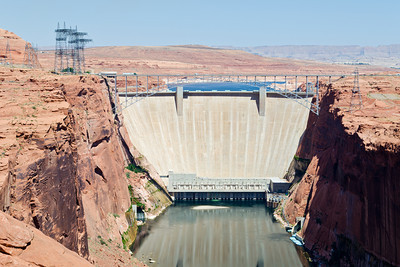
\includegraphics{best-glen-canyon-dam-view-S.jpg}}
%Glen Canyon dam
%{[}/caption{]}

\captionsetup[floatingfigure]{labelformat=empty}
\begin{floatingfigure}[r]{0.32\textwidth}
\centering
\href{http://conceptcontrol.smugmug.com/Trips/USA-and-Canada/Arizona-Toodling-1/7475075\_MrjqMc}{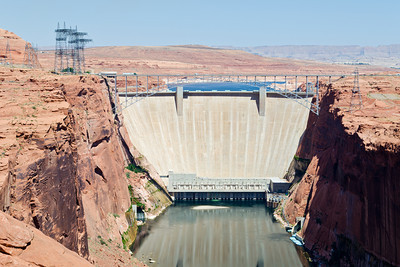
\includegraphics[width=0.30\textwidth]{best-glen-canyon-dam-view-S.jpg}}
\caption{Glen Canyon dam}
\label{fig:2818X0}
\end{floatingfigure}Last weekend I was in Page Arizona to visit my parents and catch the May
20\textsuperscript{th} 2012 annular solar eclipse. Page is a little town
that owes its existence to the construction of the Glen Canyon dam in
the early 1960s. The reservoir behind the dam, Lake Powell, has
appeared in so many movies that
\href{http://www.lakepowellrealty.net/lake-powell-movies/}{it should
collect royalties}. Charlton Heston crashed his spaceship here in the first
and
\href{http://en.wikipedia.org/wiki/Planet\_of\_the\_Apes\_(1968\_film)}{only
good Planet of the Apes movie}. John Travolta
nuked the place in \href{http://www.imdb.com/title/tt0115759/}{Broken
Arrow}. Even Jesus Christ used Lake Powell as a Dead Sea ringer in
\href{http://www.imdb.com/title/tt0059245/}{The Greatest Story Ever
Told}.

Page, the dam and Lake Powell did not disappoint. I had a great time
toodling around \href{http://conceptcontrol.smugmug.com/Trips/USA-and-Canada/Arizona-Toodling-1/7475075_MrjqMc}{shooting pictures}. I only 
had one day which was partly
devoted to the eclipse but I saw enough to give Glen Canyon an
unqualified thumbs up. If you're into rocks, desert and water this place
is \href{http://bucketlist.org/}{bucket list} material. Like MacArthur I
will return.


%{[}caption id=``'' align=``alignleft''  width=``282''{]}
%\href{http://conceptcontrol.smugmug.com/Trips/USA-and-Canada/Arizona-Toodling-1/7475075\_MrjqMc}{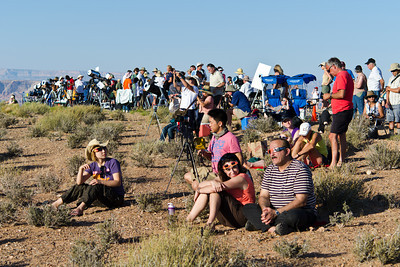
\includegraphics{wahweap-overlook-eclipse-crowd-S.jpg}}
%Wahweap Overlook eclipse fans
%{[}/caption{]}

\begin{floatingfigure}[l]{0.33\textwidth}
\centering
\href{http://conceptcontrol.smugmug.com/Trips/USA-and-Canada/Arizona-Toodling-1/7475075\_MrjqMc}{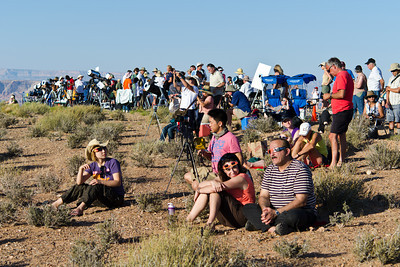
\includegraphics[width=0.30\textwidth]{wahweap-overlook-eclipse-crowd-S.jpg}}
\caption{Wahweap eclipse fans}
\label{fig:2818X1}
\end{floatingfigure}While pleased with Glen Canyon I was surprised by the large number of
people who turned out for the annular eclipse. The US park service in
conjunction with local amateur astronomers set up viewing grounds on
Wahweap Overlook and ran full size shuttle buses from the nearby Carl
Hayden dam visitor center. At least four busloads of eclipse fans were
carried to the overlook where they joined more amateur astronomers and
serious eclipse photographers that had set up dozens of telescopes and
cameras for the big show. There must have been at least four hundred
people on Wahweap Overlook and Wahweap was only one of many sites where
people set up to watch the eclipse. It's gratifying to see that when a
\emph{real star} puts on a show the audience is huge.

Before the eclipse started, and during the early phases when the Moon
was creeping on the Sun's disk, I walked around looking through
telescopes. Two scopes stood out. One expensive large aperture
\href{http://www.astronomyknowhow.com/hydrogen-alpha.htm}{Hydrogen
Alpha} scope served up gorgeous high-resolution views of the Sun. In
Hydrogen Alpha light solar prominences , filaments and photosphere
mottles are clearly visible. The big Hydrogen Alpha scope put on a good
show but bang for the buck went to a 15 dollar light funnel that a
14-year-old made by hand and attached to a small refractor. His
makeshift funnel projected the brightest and clearest white light image
of the Sun. I told him his projection was the best; he was happy to hear
it.


%{[}caption id=``attachment\_2837'' align=``alignleft''  width=``169''{]}
%\href{https://bakerjd99.files.wordpress.com/2012/05/crop-light-ring-iphone.jpg}{\includegraphics{crop-light-ring-iphone.jpg}}
%iPhone image captured by holding eclipse shades over the
%lens.
%{[}/caption{]}


As the eclipse approached the annular phase I set up my camera. I didn't
have the right filter, only a 4D neutral density, but I thought I'd give
it a try. When the light ring formed I fired off a few shots. The filter
didn't cut enough light so I immediately gave up and went to plan B.
Plan B consisted of covering the lens of my iPhone with eclipse shades
and
\href{http://bakerjd99.wordpress.com/2011/12/04/revenge-of-the-phd-camera/}{PhD'ing
it}. I took a few frames and managed to catch the ring. It was a minor
triumph of \href{http://www.iphoneography.com/}{iPhoneography}. After
that I just gawked through my eclipse shades while the Sun and Moon
wowed the masses with their dance. The crowd burst into applause when
the ring broke but, sadly, the performers declined an encore.


%{[}caption id=``'' align=``alignright''  width=``320''{]}
%\href{http://conceptcontrol.smugmug.com/Trips/USA-and-Canada/Arizona-Toodling-1/7475075\_MrjqMc}{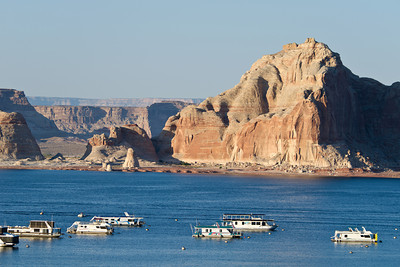
\includegraphics{lake-powell-houseboats-S.jpg}}
%Lake Powell houseboats
%{[}/caption{]}

\captionsetup[figure]{labelformat=empty}
\begin{figure}[ht]
\centering
\begin{minipage}[b]{0.46\textwidth}
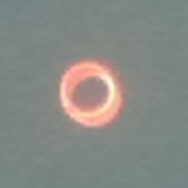
\includegraphics[width=0.30\textwidth]{lightring.jpg}\label{fig:2818X2}
\caption{iPhone image captured by holding eclipse shades over the lens}
\end{minipage}
\hspace{8pt}
\begin{minipage}[b]{0.48\textwidth}
\centering
\href{http://conceptcontrol.smugmug.com/Trips/USA-and-Canada/Arizona-Toodling-1/7475075\_MrjqMc}{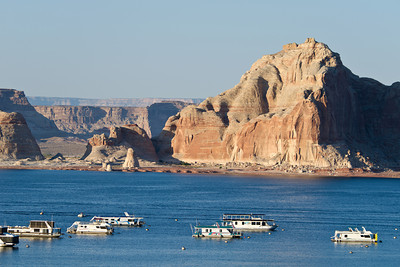
\includegraphics[width=0.90\textwidth]{lake-powell-houseboats-S.jpg}}
\caption{Lake Powell houseboats}
\label{fig:2818X3}
\end{minipage}
\end{figure}

As I have already said, annulars are not in the same awe-inspiring class
as totals but this annular, falling where it did, was special. From the
overlook you could see the lake, the dam, towering red rock formations
and of course the sky. The perfect ring of light was just the icing on
the cake of a Wahweap wow!



%\captionsetup[floatingfigure]{labelformat=empty}
%\begin{figure}[htbp]
%\begin{floatingfigure}[l]{0.25\textwidth}
%\centering
%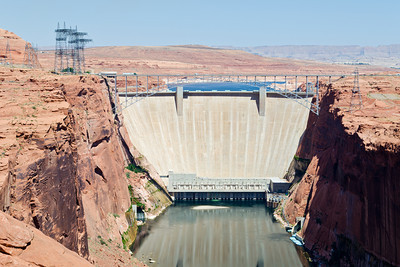
\includegraphics[width=0.23\textwidth]{best-glen-canyon-dam-view-S.jpg}
%\caption{~~~IMCAPTION~~~}
%\label{fig:2818X0}
%\end{floatingfigure}
%\end{figure}

%\captionsetup[floatingfigure]{labelformat=empty}
%\begin{figure}[htbp]
%\begin{floatingfigure}[l]{0.25\textwidth}
%\centering
%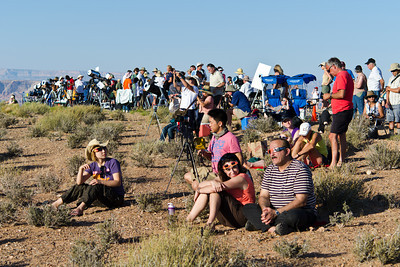
\includegraphics[width=0.23\textwidth]{wahweap-overlook-eclipse-crowd-S.jpg}
%\caption{~~~IMCAPTION~~~}
%\label{fig:2818X1}
%\end{floatingfigure}
%\end{figure}

%\captionsetup[floatingfigure]{labelformat=empty}
%\begin{figure}[htbp]
%\begin{floatingfigure}[l]{0.25\textwidth}
%\centering
%\includegraphics[width=0.23\textwidth]{crop-light-ring-iphone.jpg}
%\caption{~~~IMCAPTION~~~}
%\label{fig:2818X2}
%\end{floatingfigure}
%\end{figure}

%\captionsetup[floatingfigure]{labelformat=empty}
%\begin{figure}[htbp]
%\begin{floatingfigure}[l]{0.25\textwidth}
%\centering
%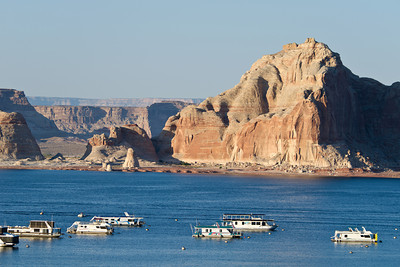
\includegraphics[width=0.23\textwidth]{lake-powell-houseboats-S.jpg}
%\caption{~~~IMCAPTION~~~}
%\label{fig:2818X3}
%\end{floatingfigure}
%\end{figure}



%\end{document}